
\documentclass[sigconf]{acmart}

\usepackage{graphicx}
\usepackage{booktabs}
\usepackage{hyperref}
\usepackage{subcaption}
\usepackage{listings}

\title{A Proxy Persona Tool For Web Viewing and Chat Interaction}

\author{Christopher B. Rauch}
\affiliation{%
  \institution{Drexel University}
  \city{Philadelphia}
  \state{PA}
  \country{USA}
}
\email{cr625@drexel.edu}

\author{Hyung Wook Choi}
\affiliation{%
  \institution{Drexel University}
  \city{Philadelphia}
  \state{PA}
  \country{USA}
}
\email{hc685@drexel.edu}

\author{Michael L. Nelson}
\affiliation{%
  \institution{Old Dominion University}
  \city{Norfolk}
  \state{VA}
  \country{USA}
}
\email{mln@cs.odu.edu}

\author{Alex H. Poole}
\affiliation{%
  \institution{Drexel University}
  \city{Philadelphia}
  \state{PA}
  \country{USA}
}
\email{ahp56@drexel.edu}

\author{Travis Reid}
\affiliation{%
  \institution{Old Dominion University}
  \city{Norfolk}
  \state{VA}
  \country{USA}
}
\email{treid003@odu.edu}

\author{Michele C. Weigle}
\affiliation{%
  \institution{Old Dominion University}
  \city{Norfolk}
  \state{VA}
  \country{USA}
}
\email{mweigle@cs.odu.edu}

\author{Mat Kelly}
\affiliation{%
  \institution{Drexel University}
  \city{Philadelphia}
  \state{PA}
  \country{USA}
}
\email{mkelly@drexel.edu}

\begin{abstract}
This demo presents an interactive proxy tool designed to capture, inspect, and preserve personalized online activity in real-time browsing sessions. The system offers researchers and archivists a method to analyze the behaviors and presence of ads and other dynamic content during web interactions. The tool can be extended to provide context to Large Language Models that leverages the personalization options available in the major models and also allows persona information to be passed as additional context.
\end{abstract}

\keywords{web archiving, advertisements, proxy server, personalization}

\begin{document}
\begin{teaserfigure}
  \centering
  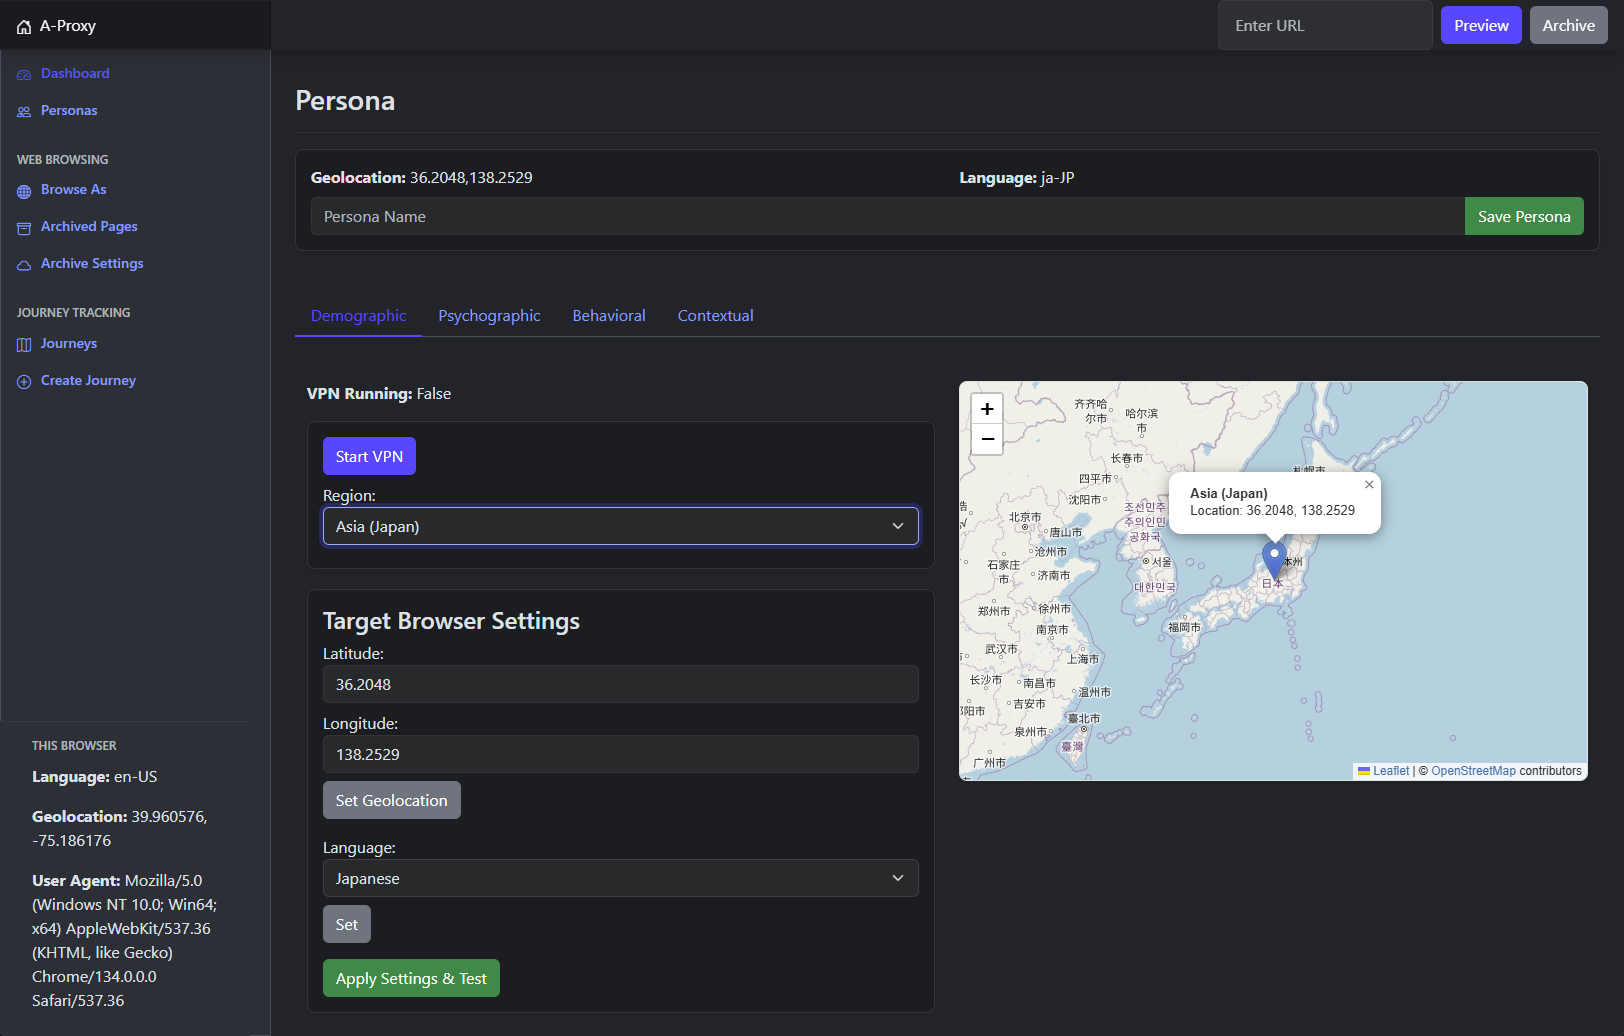
\includegraphics[width=\textwidth]{persona-teaser.png}
  \caption{Interface of the proxy system showing persona-level customization, including geolocation, language, and behavioral settings. The system enables fine-grained control over browser characteristics to simulate user experiences during web archiving or ad tracking.}
  \Description{Screenshot of A-Proxy interface showing persona settings, VPN toggle, and browser controls including geolocation and language.}
  \label{fig:persona}
\end{teaserfigure}
\maketitle


\section{Introduction}
Web advertisements are personalized according to marketing categories...

There are tools for mocking browser interactions but nothing specifically designed for archivists

Related work

\section{System Overview}
Local HTTP proxy that intercepts and logs ad-related requests during a browsing session. Users direct their browser traffic through the proxy, which records third-party requests, DOM changes, and visual captures of ad content.

\section{System Architecture}
Core components

Database design

VPN Integration

System Diagram.

\section{Demo Scenario}
This tool is suited for digital preservationists, researchers conducting web-based content audits, and scholars studying online influence. For example, one can use the proxy to inspect how ad content differs across user personas or to compare live versus archived versions of the same page.

\section{Implementation}
The proxy is written in Python and uses a combination of proxy server and browser testing tools for traffic interception and modification. Captured ad content is rendered and stored locally in a structured format. The system integrates with headless browsers to automate browsing sessions for reproducibility.

The source code is available at: \url{https://github.com/savingads/a-proxy}

A demonstration video is accessible at: \url{[INSERT VIDEO LINK HERE]}

\section{Conclusion and Future Work}
Future work includes support for mobile traffic, real-time annotation, and integration with archival platforms and llms

\bibliographystyle{ACM-Reference-Format}
\bibliography{software}

\end{document}
